\documentclass[12pt]{article}

\usepackage{fullpage,soul,graphicx,esvect,stoversymb,changepage}
%                              ^ for underline: \ul{...}
%\everymath{\displaystyle}
\pagenumbering{gobble}

\usepackage{multicol}
\usepackage[many]{tcolorbox}
\usepackage{tikz}
\usepackage{booktabs}
\usepackage[inline]{enumitem}
\usepackage{pgfplots}


\usepackage[letterpaper, margin=0.5in, top=0.5in, bottom=1in]{geometry}

%\setenumerate{itemsep=0.25in}
\setlist[enumerate,1]{leftmargin=0.2in,itemsep=0.25in}%, itemsep=1.25in}
\setlist[enumerate,2]{label=(\roman*),leftmargin=0.375in,itemsep=0.125in}

\graphicspath{ {./../img/} }
\DeclareGraphicsExtensions{.pdf}

\newcommand{\scratch}{\newpage\thispagestyle{empty}\begin{center}Scratch Paper\end{center}}
\newcommand{\sol}{\par\vspace{4.5mm}\hspace{-4.5mm}\textsc{Solution:}}
\newcommand{\hint}[1]{\textbf{Hint}: #1}
\newcommand{\hints}[1]{\textbf{Hints}: #1}
\newcommand{\note}[1]{\textbf{Note}: #1}
\newcommand{\why}{\textit{why?}}
\newcommand{\ptsea}[1]{(\textit{#1 pts ea.})}
\newcommand{\axes}[1]{\begin{center}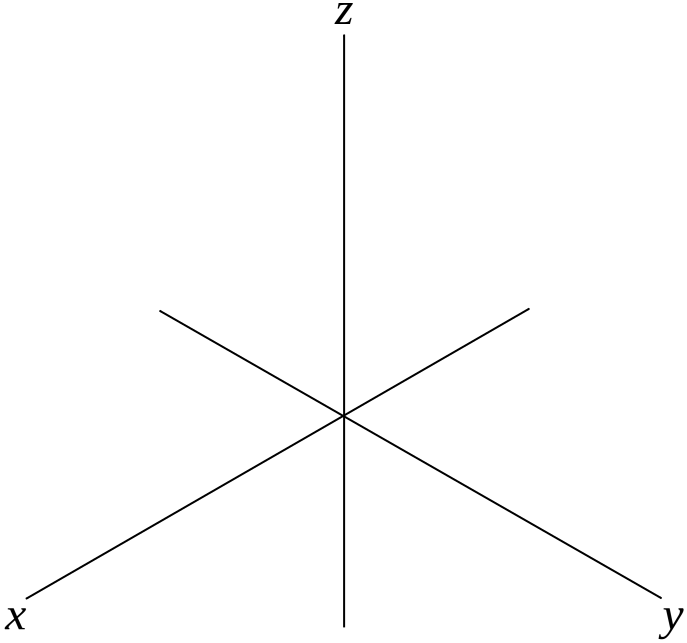
\includegraphics[scale=#1]{3DAxes}\end{center}}
\newcommand{\axespt}[1]{\begin{center}\includegraphics[scale=#1]{3DAxesWithPoint}\end{center}}
\newcommand{\pic}[2]{\begin{center}\includegraphics[scale=#1]{#2}\end{center}}
\newcommand{\comps}[1]{\langle #1_1,#1_2,#1_3\rangle}
\newcommand{\compslong}[3]{\langle #1, #2, #3\rangle}
\newcommand{\resultbox}[1]{\begin{center}
		\begin{tcolorbox}[
			enhanced,
			colback=white,
			colframe=white,
			boxrule=0.5pt,
			arc=0pt,
			top=3mm,
			bottom=3mm, 
			width=7in%,
			%			grow to left by=0.5in,
			]
			%\centering
			#1
		\end{tcolorbox}
\end{center}}

\begin{document}
	\begin{flushright}{\large \textbf{\S16.7--\S16.9 Review Problems}} \hfill Name: \line(1,0){200}\end{flushright}
	\resultbox{\textbf{Note:} This isn't for a grade and there is no due date. Also, if your goal is to focus on the new material, you should do problems 2--5 first.}
	\begin{enumerate}
		\item Evaluate the surface integral 
		$$\iint\limits_F \vect{F}\cdot d\vect{S},$$ where $\vect{F}(x,y,z)=xy\,\vect{i}+3x^2\,\vect{j}+xz\,\vect{k}$ and where $F$ is the surface $z=xe^y$, $0\leq x\leq 1$, $0\leq y\leq 1$ with upward orientation.
		\item Use Stokes' theorem to evaluate each of the following.
			\begin{enumerate}
				\item $\iint_F\Curl\vect{F}\cdot d\vect{S},$
				where $\vect{F}=\langle2x\cos{2z},e^y\sin{z},x^2ye^y\rangle$ and $F$ is the hemisphere $x^2+y^2+z^2=4$, $z\geq 0$, oriented upward.
				\item $\oint_C\vect{F}\cdot d\vect{r}$, where $\vect{F}(x,y,z)=(x+y^2)\,\vect{i}+(y+z^2)\,\vect{j}+(z+x^2)\,\vect{k}$ and where $C$ is the triangle with vertices $(2,0,0)$, $(0,2,0)$, and $(0,0,2)$.
			\end{enumerate}
		\item Verify that Stokes' theorem is true for the vector field $\vect{F}=\langle y, z, x\rangle$ and the surface $F$ equal to the hemisphere $x^2+y^2+z^2=1$, $z\geq 0$, oriented upward. 
		
		\hint{$\sin^2(x)=\frac{1}{2}(1-\cos{2x})$. Also you can parametrize $F$ as 
		$$\vect{r}(u,v)=\langle \cos(u)\sin(v),\sin(u)\sin(v),\cos(v)\rangle\quad\quad(0\leq u\leq 2\pi, 0\leq v\leq \pi/2),$$
		which is like spherical coordinates with $\rho=1$ \textit{except} that $dA=du\,dv$ without a pesky $\sin(v)$ Jacobian-thing in there.}
		\item Use the divergence theorem to compute each of the following.
			\begin{enumerate}
				\item The flux of $\vect{F}=\langle x^2\sin{y},x\cos{y},-xz\sin{y}\rangle$ across the ``fat sphere'' $F$ equal to $x^8+y^8+z^8=8$.
				\item $\iint_F\vect{F}\cdot d\vect{S}$, where $\vect{F}=(\cos{z}e^{e^z}+xy^2)\,\vect{i}+z\cos{x}\sin{xz}e^{-z}\,\vect{j}+(\sin{y}+x^2z)\vect{k}$ and where $F$ is the surface of the solid bounded by the paraboloid $z=x^2+y^2$ and the plane $z=4$. 
				
				\hint{Use cylindrical coordinates}.
			\end{enumerate}
		\item Verify that the divergence theorem is true for the vector field $\vect{F}=\langle x^2,xy,z\rangle$ and the solid $E$ bounded by the paraboloid $z=4-x^2-y^2$ and the $xy$-plane.
	\end{enumerate}
\end{document}